\chapter[SCP-127 活体枪]{
    SCP-127 The Living Gun\\
    SCP-127 活体枪
}

\label{chap:SCP-127}

\begin{figure}[H]
    \centering
    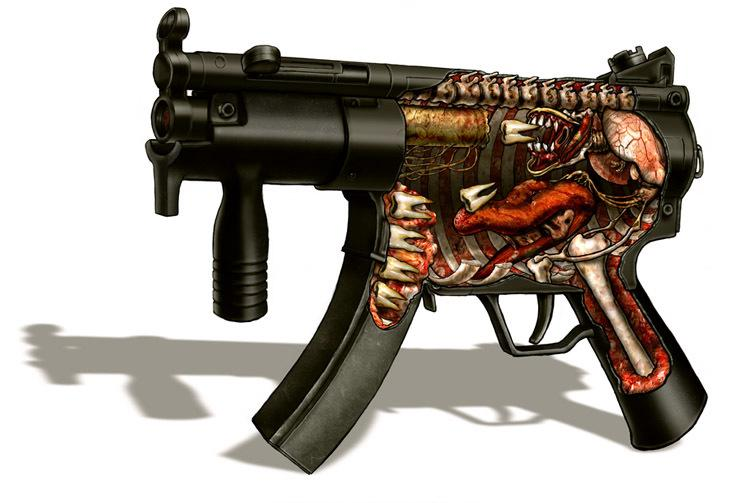
\includegraphics[width=0.5\linewidth]{images/SCP-127.jpg}
    \caption*{对于SCP-127内部结构的艺术分析图}
\end{figure}

\bb{项目编号:}SCP-127

\bb{项目等级:}Safe

\bb{特殊收容措施}:SCP-127在慎重考虑后认为并不比同型的普通枪支更为危险。尽管如此,考虑到它令人惊奇的属性,它在不使用的情况下它被浸泡在富含钙和蛋白质的水里,放在7-C武器库。这个时候,只有SCP-127的指定研究小组才有权限使用它。

\bb{描述:}SCP-127,一眼看上去,像是一支标准MP5K微型冲锋枪。测试显示它并不使用外装式金属子弹,整支武器都是有机化和活生生的。武器的子弹最初看起来就像人类的牙齿。尽管如此,DNA测试显示“子弹”并不属于地球上任何一个物种。

SCP-127可以切换为两个模式:半自动和全自动(在两个模式之间切换的时候能听见呻吟声)。在打光武器的“弹匣”后(60发装型号弹匣),它会在3-5天内出新长出子弹来。试拿下弹匣的努力失败了,似乎这个弹匣是完全和武器永久镶嵌在一起得。

SCP-127看上去没有任何生殖的能力(扫描显示没有任何生殖器官)并且除了水,钙,蛋白质外不需要任何其他营养。

SCP-127最初在James █████████████先生的房子里。 █████████████先生在1991年11月17日晚间被发现死于心脏病。验尸官报告显示 █████████████先生死于11月8日早上的某个时候,不过直到一周后才有人注意到此人消失。没有发现他死于任何并发症或者通常环境问题。由于他拥有大量的枪支收藏,ATF(美国烟酒枪炮及爆炸物管理局)和FBI被指示来收集他的武器。SCP-127在测试和编码过程中被发现,并马上被SCP特工回收。

\bb{附录}:于1991年██月█日重新将等级编制为Safe。
